\chapter{Radiation from Hot and Fast Particles}
\label{ch:fastparticles}

\newcommand{\FifteenSyncXpeak}{0.29}
\newcommand{\FifteenSyncSlope}{-0.752}
\newcommand{\FifteenSyncSlopeLow}{0.32}
\newcommand{\FifteenSyncP}{2.5}


Stars shine because they are hot and opaque, and their light is close to the light of a blackbody (Chapter~\ref{ch:radiation}). Much of the sky does not shine that way. The gas between the galaxies of a cluster glows in X-rays, though it is far too thin to be opaque. Radio galaxies send out spectra that fall smoothly as a power of the frequency over many decades, which no single temperature can make. A quasar outshines its whole galaxy from a region a few light-days across.

All of this light comes from charges that are pushed about, by ions, by magnetic fields, or by collisions with fast electrons. One formula from electromagnetism, the power radiated by an accelerated charge, gives every spectrum in the chapter when it is combined with the six principles. Fast particles need one more tool, the Lorentz transformation, which we write as a matrix.

% ==============================================================================
\section{An Accelerated Charge Radiates}
\label{fp:sec:larmor}

Chapter~\ref{ch:ism} used the power radiated by a shaken electron to find the Thomson cross-section, Eq.~\eqref{eq:thomson_cross_section}.

There the electron was driven gently by a passing wave and always moved slowly. In hot gas and in jets, electrons are flung about by ions, spun round magnetic field lines, and move close to the speed of light. We need to know how much they radiate, and how motion near $c$ changes what an observer sees.

Hold one end of a long rope lying on the floor. If you keep your hand still, or move it at a steady speed, nothing travels down the rope. If you jerk your hand, a pulse runs away along it, and the pulse carries energy that your arm supplied. A harder jerk sends a bigger pulse. What matters is how suddenly the hand changes its speed, not how fast it moves.

A charge does the same with its electric field. An electron passing close to a proton is jerked sideways once. An electron in a magnetic field is jerked all the time, as it is turned round in a circle. Each jerk sends out a pulse of electromagnetic field that carries energy away (P1). The power depends on the square of the acceleration, and for an electron it is a small loss per turn unless the acceleration is extreme (P6).

The classical hydrogen atom in numbers. An electron circling a proton at the Bohr radius $5.29\times10^{-11}\,\mathrm m$ has an acceleration of $9.0\times10^{22}\,\mathrm{m\,s^{-2}}$ and would radiate $4.7\times10^{-8}\,\mathrm W$. Its energy of $13.6\,\mathrm{eV}$ would last $4.7\times10^{-11}\,\mathrm s$, while one orbit takes $1.5\times10^{-16}\,\mathrm s$. It would lose only $1.6\times10^{-6}$ of its energy per orbit. Quantum mechanics stops the real atom from radiating at all, but the ratio shows that radiation drains a moving charge slowly compared with its own motion.

The picture is a shell of field spreading out from the charge at the speed of light, strongest at right angles to the acceleration and zero along it.

The same formula runs radio antennas, X-ray tubes and the synchrotron light sources of laboratories. It gave the Rayleigh and Thomson scattering of Chapter~\ref{ch:ism}. It uses P1 (the field carries energy) and P6 (the rate of radiation compared with the rate of motion). It gives the radiated power, how large it is, and how it changes when the charge moves near the speed of light.

\paragraph{The Larmor formula.} A charge $e$ moving slowly, $v\ll c$, with acceleration $\dot{\vec v}$ radiates the power
\begin{equation}
	\mathcal P=\frac{e^2\,|\dot{\vec v}|^2}{6\pi\varepsilon_0c^3},\qquad
	\dv{\mathcal P}{\Omega}=\frac{e^2\,|\dot{\vec v}|^2}{16\pi^2\varepsilon_0c^3}\,\sin^2\Theta ,
	\label{fp:eq:larmor}
\end{equation}
where $\Theta$ is the angle between the acceleration and the direction of emission. These are quoted from electromagnetism. The second form integrates to the first, since $\int\sin^2\Theta\,d\Omega=8\pi/3$. The pattern is the same in a direction and in the opposite direction, so the radiation carries away energy but no net momentum.

\paragraph{How fast a charge loses its energy.} To compare the radiated energy with the energy of the motion, take an electron of mass $m_e$ oscillating as $x=x_0\cos\omega t$ (P6). Its acceleration is $\dot v=-\omega^2x$, its energy is $\tfrac12m_e\omega^2x_0^2$, and in one radian of its motion, a time $1/\omega$, it radiates $\avg{\mathcal P}/\omega$.
\begin{align}
	\frac{\text{energy radiated per radian}}{\text{energy of the motion}}
	&\eqby{1} \frac{e^2\,\omega^4x_0^2/(12\pi\varepsilon_0c^3)}{\omega\cdot\tfrac12m_e\omega^2x_0^2} \nonumber\\
	&\eqby{2} \omega\,\frac{e^2}{6\pi\varepsilon_0m_ec^3}
	\eqby{3} \omega\,t_e .
\end{align}
\begin{explain}
	\item Eq.~\eqref{fp:eq:larmor} with $|\dot v|^2=\omega^4x_0^2\cos^2\omega t$, whose average over a cycle is $\omega^4x_0^2/2$.
	\item The factors $x_0^2$ and $\omega^3$ cancel.
	\item Define the \textbf{radiation time} $t_e$ below.
\end{explain}
\begin{equation}
	\boxed{t_e=\frac{e^2}{6\pi\varepsilon_0m_ec^3}=\frac23\,\frac{r_e}{c}=6.27\times10^{-24}\,\mathrm s .}
	\label{fp:eq:tau_e}
\end{equation}
Here $r_e$ is the classical electron radius of Eq.~\eqref{eq:thomson_cross_section}, so $t_e$ is two thirds of the time light takes to cross it. An electron loses the fraction $\omega t_e$ of its energy per radian, and $\omega t_e\ll1$ for any motion short of $10^{23}$ turns per second. We may therefore work out the motion of a charge as if it did not radiate, and then add Larmor's power. This is how every spectrum below is found.

\paragraph{Fast charges and the boost matrix.} Let a frame move with the charge at speed $\beta c$ along $x$ relative to the frame of the observer. We call the first the charge's frame (primed) and the second the lab. The lab components of an event or of a four-momentum follow from those in the charge's frame by the boost
\begin{equation}
	\begin{pmatrix}ct\\x\\y\end{pmatrix}=\Lambda(\beta)\begin{pmatrix}ct'\\x'\\y'\end{pmatrix},\qquad
	\Lambda(\beta)=\begin{pmatrix}\gamma_L&\gamma_L\beta&0\\ \gamma_L\beta&\gamma_L&0\\0&0&1\end{pmatrix},\qquad
	\gamma_L=\frac{1}{\sqrt{1-\beta^2}} ,
	\label{fp:eq:boost}
\end{equation}
with the $z$ component unchanged and left out. The same matrix acts on an energy and momentum written as $(E/c,\ \text{momentum along }x,\ \text{momentum along }y)$. Its inverse is $\Lambda(-\beta)$, the boost from the lab into the charge's frame. Here $\gamma_L$ is the \textbf{Lorentz factor}, with the subscript to keep it apart from the adiabatic exponent $\gamma$.

\paragraph{The power is the same in both frames.} In its own frame the charge is momentarily at rest, so Larmor's formula holds there. In a time $dt'$ it radiates an energy $dE'$ and, by the symmetry of Eq.~\eqref{fp:eq:larmor}, no net momentum. The emissions happen at the charge, $x'=y'=0$. Boosting the energy-momentum and the time interval to the lab,
\begin{align}
	\Lambda(\beta)\begin{pmatrix}dE'/c\\0\\0\end{pmatrix}
	&\eqby{1} \begin{pmatrix}\gamma_L\,dE'/c\\ \gamma_L\beta\,dE'/c\\0\end{pmatrix},
	&
	\Lambda(\beta)\begin{pmatrix}c\,dt'\\0\\0\end{pmatrix}
	&\eqby{1} \begin{pmatrix}\gamma_L\,c\,dt'\\ \gamma_L\beta\,c\,dt'\\0\end{pmatrix}, \nonumber\\
	\implies\quad dE&=\gamma_L\,dE', & dt&=\gamma_L\,dt' .
\end{align}
\begin{explain}
	\item The matrix of Eq.~\eqref{fp:eq:boost} times a vector with only its first entry non-zero is that entry times the first column.
\end{explain}
The factors $\gamma_L$ cancel in the ratio,
\begin{equation}
	\boxed{\mathcal P=\dv{E}{t}=\dv{E'}{t'}=\frac{e^2\,|\dot{\vec v}'|^2}{6\pi\varepsilon_0c^3},}
	\label{fp:eq:power_invariant}
\end{equation}
where $\dot{\vec v}'$ is the acceleration in the charge's own frame. To find the power of a fast charge we find its acceleration in its own frame and use Larmor's formula there. The power that an observer receives is a different thing, since the observer also sees the pulses squeezed together in time. That squeezing sets the frequencies of synchrotron light in Section~\ref{fp:sec:sync}.

\paragraph{Beaming.} A photon of frequency $\nu'$ emitted in the charge's frame at angle $\theta'$ to the direction of motion has four-momentum $(h\nu'/c)(1,\cos\theta',\sin\theta')$. In the lab it has frequency $\nu$ and angle $\theta$,
\begin{align}
	\frac{h\nu}{c}\begin{pmatrix}1\\ \cos\theta\\ \sin\theta\end{pmatrix}
	&\eqby{1} \Lambda(\beta)\,\frac{h\nu'}{c}\begin{pmatrix}1\\ \cos\theta'\\ \sin\theta'\end{pmatrix}
	\eqby{2} \frac{h\nu'}{c}\begin{pmatrix}\gamma_L(1+\beta\cos\theta')\\ \gamma_L(\cos\theta'+\beta)\\ \sin\theta'\end{pmatrix} \nonumber\\
	\implies\quad \tan\theta
	&\eqby{3} \frac{\sin\theta'}{\gamma_L(\cos\theta'+\beta)},\qquad
	\nu \eqby{4} \gamma_L(1+\beta\cos\theta')\,\nu' .
	\label{fp:eq:beaming}
\end{align}
\begin{explain}
	\item The boost \eqref{fp:eq:boost} applied to the photon's four-momentum.
	\item The matrix product, row by row.
	\item The third row divided by the second.
	\item The first row.
\end{explain}
A photon sent sideways in the charge's frame, $\theta'=\pi/2$, has $\tan\theta=1/(\gamma_L\beta)$ in the lab. All the light of the forward half of the charge's frame, which is half of all its light, lands within this angle,
\[
\boxed{\theta\lesssim\frac{1}{\gamma_L}\qquad(\gamma_L\gg1).}
\]
An electron with $\gamma_L=10$ throws half its light into a cone of half-angle $6^\circ$ about its velocity (Figure~\ref{fp:fig:beaming}). The frequency in Eq.~\eqref{fp:eq:beaming} at $\theta'=0$ is $\gamma_L(1+\beta)\nu'=\sqrt{(1+\beta)/(1-\beta)}\,\nu'$, the exact Doppler shift of an approaching source, Eq.~\eqref{eq:doppler_relativistic}, as it must be.

\begin{figure}[htbp]
	\centering
	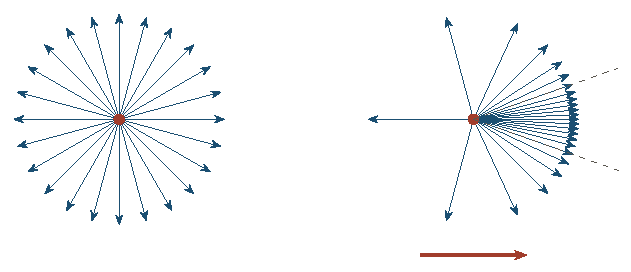
\includegraphics{fig_ch15_beaming.pdf}
	\caption{Photons emitted at equal steps of angle in the frame of the emitter (left), and the same photons in a frame where the emitter moves to the right with $\gamma_L=3$ (right). The dashed lines mark the angle $\tan\theta=1/(\gamma_L\beta)$.}
	\label{fp:fig:beaming}
\end{figure}

% ==============================================================================
\section{Bremsstrahlung}
\label{fp:sec:brems}

The hot gas that fills a cluster of galaxies is at about $7\times10^7\,\mathrm K$, set by the depth of the cluster's gravitational well (Problem~\ref{sg:prob:cluster}), and the gas is fully ionised.

It is also so thin that light crosses it freely, so by Eq.~\eqref{rad:eq:slab} it does not shine as a blackbody. Fully ionised gas has no bound electrons to make lines. Something else must make its light.

Think of rain on the roof of a car. Each drop makes a short click, and a short click contains every pitch up to about one over its length. The sound inside the car is the number of drops striking per second times the energy of each click. Heavier rain is louder, and the sharpest clicks give the highest pitches.

In hot gas the drops are electrons and the roof is the ions. Each electron that passes an ion is jerked once and sends out one pulse of light, as in Section~\ref{fp:sec:larmor}. The gas glows with the sum of countless such pulses. The idea is to find the spectrum of one encounter and then count the encounters, over impact parameters (P6) and over the Maxwell distribution of speeds (P3).

The cluster in numbers. Its electrons have $k_BT=6.0\,\mathrm{keV}$. No photon can carry more energy than the electron that made it (P1), so the spectrum must end near $6\,\mathrm{keV}$, at $1.5\times10^{18}\,\mathrm{Hz}$, in X-rays.

The picture is an electron flying past an ion, its path bent slightly near closest approach, with a flash of light sent out at the bend.

The same process is the braking radiation (\emph{Bremsstrahlung}) of an X-ray tube. It makes the radio glow of ionised hydrogen around hot stars, the X-rays of solar flares and of clusters. Run backwards, as absorption, it is the opacity of stellar interiors. It uses P1, P3, P6 and, for absorption, the detailed balance of P4. It gives the emissivity of a hot plasma, its cooling rate and cooling time, and its absorption.

\paragraph{A gas of free charges.} Before counting encounters one at a time, we check that each is a meeting of two particles and not a crowd. Put an ion of charge $Z_ie$ at the origin, in gas of electron density $n_e$ at temperature $T$. Electrons gather near it with the Boltzmann weight $e^{e\phi/k_BT}$, where $\phi$ is the electric potential (P3). Poisson's equation, the electric version of Eq.~\eqref{pr:eq:poisson}, then reads, away from the ion,
\begin{align}
	\nabla^2\phi
	&\eqby{1} -\frac{e}{\varepsilon_0}\Big(Z_in_i-n_e\,e^{e\phi/k_BT}\Big) \nonumber\\
	&\eqby{2} \frac{n_ee^2}{\varepsilon_0k_BT}\,\phi
	\eqby{3} \frac{\phi}{\lambda_D^2} \nonumber\\
	\implies\quad \phi
	&\eqby{4} \frac{Z_ie}{4\pi\varepsilon_0r}\,e^{-r/\lambda_D} .
\end{align}
\begin{explain}
	\item The charge density is that of the ions, $Z_ien_i$, minus that of the electrons. The ions are heavy and stay spread evenly on the scale considered.
	\item Far from the ion $e\phi\ll k_BT$, so $e^{e\phi/k_BT}\approx1+e\phi/k_BT$. The gas is neutral on average, $Z_in_i=n_e$.
	\item Define the \textbf{Debye length} $\lambda_D$ below.
	\item The spherically symmetric solution that matches the bare ion's potential at small $r$. Substituting it back gives $\nabla^2\phi=\phi/\lambda_D^2$.
\end{explain}
\begin{equation}
	\boxed{\lambda_D=\sqrt{\frac{\varepsilon_0k_BT}{n_ee^2}}=\frac{\sqrt{k_BT/m_e}}{2\pi\nu_p} .}
	\label{fp:eq:debye}
\end{equation}
The second form uses the plasma frequency of Eq.~\eqref{re:eq:plasma_frequency}. The Debye length is the distance a thermal electron covers in one plasma oscillation. Beyond it, the field of any charge is cancelled by the cloud it gathers. In cluster gas, $n_e=10^3\,\mathrm{m^{-3}}$ and $T=7\times10^7\,\mathrm K$ give $\lambda_D=18\,\mathrm{km}$, with $2.5\times10^{16}$ electrons inside a sphere of that radius. Gas round a hot star, $n_e=10^8\,\mathrm{m^{-3}}$ and $T=10^4\,\mathrm K$, gives $\lambda_D=0.7\,\mathrm m$ and $1.4\times10^8$ electrons (P6). With so many charges inside each Debye sphere, the screening is a smooth average, and an electron feels one ion strongly only when it passes far closer than $\lambda_D$. Such a gas is a \textbf{plasma}. It behaves as an ideal gas, its encounters can be counted one at a time, and by Chapter~\ref{ch:resolution} it lets no radiation below $\nu_p$ through.

\paragraph{One encounter.} An electron of speed $v$ passes an ion of charge $Z_ie$ at impact parameter $b$. Its path bends only slightly, so we take it as a straight line, with closest approach at $t=0$. The force across the path is $Z_ie^2b/[4\pi\varepsilon_0(b^2+v^2t^2)^{3/2}]$. The total sideways kick is
\begin{align}
	\Delta v
	&\eqby{1} \frac{Z_ie^2b}{4\pi\varepsilon_0m_e}\int_{-\infty}^{\infty}\frac{dt}{(b^2+v^2t^2)^{3/2}}
	\eqby{2} \frac{2Z_ie^2}{4\pi\varepsilon_0m_e\,bv} .
	\label{fp:eq:kick}
\end{align}
\begin{explain}
	\item Newton's law across the path, integrated over the passage.
	\item $\int_{-\infty}^\infty dt/(b^2+v^2t^2)^{3/2}=2/(b^2v)$.
\end{explain}
To find how the radiated energy is spread over frequency, write the acceleration through its Fourier transform $\tilde{\dot v}(\omega)=\int\dot v\,e^{i\omega t}dt$. For a real signal, Parseval's theorem gives $\int\dot v^2dt=\tfrac1\pi\int_0^\infty|\tilde{\dot v}|^2d\omega$, so the total energy $W$ of the pulse is
\begin{align}
	W
	&\eqby{1} \frac{e^2}{6\pi\varepsilon_0c^3}\int_{-\infty}^\infty\dot v^2\,dt
	\eqby{2} \int_0^\infty\frac{e^2\,|\tilde{\dot v}(\omega)|^2}{6\pi^2\varepsilon_0c^3}\,d\omega \nonumber\\
	\implies\quad \dv{W}{\omega}
	&\eqby{3} \frac{e^2\,(\Delta v)^2}{6\pi^2\varepsilon_0c^3}\Big[uK_1(u)\Big]^2,\qquad u=\frac{\omega b}{v} .
\end{align}
\begin{explain}
	\item Larmor's power \eqref{fp:eq:larmor} integrated over the passage.
	\item Parseval's theorem.
	\item The transform of the force law above is $\tilde{\dot v}=\Delta v\,uK_1(u)$, with $K_1$ a modified Bessel function. The component of the acceleration along the path changes sign during the passage and adds much less at low frequency, so it is dropped.
\end{explain}
The factor $uK_1(u)$ is $1$ for $u\ll1$ and falls as $e^{-u}$ for $u\gg1$. So
\begin{equation}
	\boxed{\dv{W}{\omega}\approx\frac{e^2}{6\pi^2\varepsilon_0c^3}\left(\frac{2Z_ie^2}{4\pi\varepsilon_0m_e\,bv}\right)^2\quad\text{for }\omega\lesssim\frac vb,\qquad\approx0\ \text{above}.}
	\label{fp:eq:one_encounter}
\end{equation}
The pulse lasts about $b/v$, and a pulse holds every frequency up to the inverse of its length (P6). Below that the spectrum is flat. This is the click on the roof.

\paragraph{Counting encounters.} In a unit volume, electrons of speed $v$ meet ions with impact parameters between $b$ and $b+db$ at the rate $n_en_iv\,2\pi b\,db$. Each such encounter gives Eq.~\eqref{fp:eq:one_encounter} at the frequencies $\omega<v/b$, that is for $b<v/\omega$.
\begin{align}
	\frac{dW}{dt\,dV\,d\omega}
	&\eqby{1} n_en_iv\int_{b_{\min}}^{b_{\max}}2\pi b\,\dv{W}{\omega}\,db \nonumber\\
	&\eqby{2} n_en_iv\,2\pi\,\frac{e^2}{6\pi^2\varepsilon_0c^3}\left(\frac{2Z_ie^2}{4\pi\varepsilon_0m_ev}\right)^2\int_{b_{\min}}^{b_{\max}}\frac{db}{b} \nonumber\\
	&\eqby{3} \frac{16}{3}\,\frac{Z_i^2e^6}{(4\pi\varepsilon_0)^3c^3m_e^2}\,\frac{n_en_i}{v}\,\ln\frac{b_{\max}}{b_{\min}} .
	\label{fp:eq:brems_v}
\end{align}
\begin{explain}
	\item Rate of encounters times the energy each gives per unit frequency.
	\item Eq.~\eqref{fp:eq:one_encounter}. Its $b^{-2}$ against the $b$ of the ring leaves $db/b$.
	\item Collect constants. $2\pi\times4/(6\pi^2)=4/(3\pi)$, and $e^2/\varepsilon_0=4\pi e^2/(4\pi\varepsilon_0)$.
\end{explain}
Distant encounters stop counting at $b_{\max}=v/\omega$, where the pulse becomes too slow to make the frequency $\omega$. Close ones stop at the larger of two lengths, the distance $Z_ie^2/(4\pi\varepsilon_0m_ev^2)$ where the kick is no longer small, and the electron's quantum wavelength $\hbar/(m_ev)$. The logarithm changes slowly. The full quantum calculation replaces $\ln(b_{\max}/b_{\min})$ by $(\pi/\sqrt3)\,\bar g$, where the \textbf{Gaunt factor} $\bar g$ is of order one. Slow electrons radiate more, as $1/v$, because they spend longer near each ion.

\paragraph{Averaging over the Maxwell distribution.} In gas at temperature $T$ the electrons have the Maxwell distribution of Eq.~\eqref{pr:eq:ideal_gas}, with $4\pi v^2e^{-m_ev^2/2k_BT}dv$ electrons per speed interval (P3). Only electrons with $\tfrac12m_ev^2\ge h\nu$ can make a photon of energy $h\nu$ (P1). The average of $1/v$ that Eq.~\eqref{fp:eq:brems_v} needs is
\begin{align}
	\avg{\frac1v}
	&\eqby{1} \frac{\int_{v_{\min}}^\infty v\,e^{-m_ev^2/2k_BT}\,dv}{\int_0^\infty v^2\,e^{-m_ev^2/2k_BT}\,dv}
	\eqby{2} \frac{(k_BT/m_e)\,e^{-h\nu/k_BT}}{\sqrt{\pi/2}\,(k_BT/m_e)^{3/2}}
	\eqby{3} \sqrt{\frac{2m_e}{\pi k_BT}}\;e^{-h\nu/k_BT} .
\end{align}
\begin{explain}
	\item The weight $v^2$ of the Maxwell distribution times $1/v$, normalised. The lower limit is $\tfrac12m_ev_{\min}^2=h\nu$.
	\item The two Gaussian integrals, with $m_ev_{\min}^2/2k_BT=h\nu/k_BT$.
	\item Simplify.
\end{explain}
Putting this into Eq.~\eqref{fp:eq:brems_v}, using $d\omega=2\pi\,d\nu$, and writing the result as $4\pi j_\nu$ with $j_\nu$ the emissivity per steradian of Chapter~\ref{ch:radiation},
\begin{equation}
	\boxed{4\pi j_\nu=\frac{32\pi^2}{3\sqrt3}\,\frac{Z_i^2e^6}{(4\pi\varepsilon_0)^3c^3m_e^2}\sqrt{\frac{2m_e}{\pi k_BT}}\;\bar g\,n_en_i\,e^{-h\nu/k_BT}
	=6.8\times10^{-51}\,Z_i^2\,\bar g\,\frac{n_en_i}{\sqrt T}\,e^{-h\nu/k_BT},}
	\label{fp:eq:brems_jnu}
\end{equation}
in $\mathrm{W\,m^{-3}\,Hz^{-1}}$, with $n_e,n_i$ in $\mathrm{m^{-3}}$ and $T$ in kelvin. The spectrum is flat, apart from the slow change of $\bar g$, up to $h\nu\approx k_BT$, and then falls exponentially (Figure~\ref{fp:fig:brems}). The place where it turns down measures the temperature of the gas directly. At low frequencies hotter gas is fainter, as $T^{-1/2}$, because its electrons are faster and spend less time near each ion.

\begin{figure}[htbp]
	\centering
	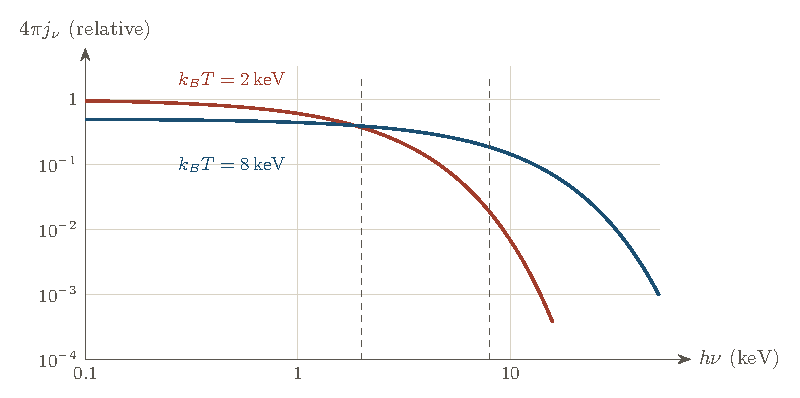
\includegraphics{fig_ch15_brems_spectrum.pdf}
	\caption{Bremsstrahlung emissivity $4\pi j_\nu\propto T^{-1/2}e^{-h\nu/k_BT}$ against photon energy, for the same electron and ion densities at $k_BT=2\,\mathrm{keV}$ and $8\,\mathrm{keV}$, with $\bar g$ held fixed. Dashed lines mark $h\nu=k_BT$.}
	\label{fp:fig:brems}
\end{figure}

\paragraph{Cooling.} Integrating over frequency, $\int_0^\infty e^{-h\nu/k_BT}d\nu=k_BT/h$, so the power radiated per unit volume is
\begin{equation}
	\boxed{4\pi\int_0^\infty j_\nu\,d\nu=6.8\times10^{-51}\,\frac{k_B}{h}\,Z_i^2\,\bar g\,n_en_i\sqrt T=1.4\times10^{-40}\,Z_i^2\,\bar g\,n_en_i\sqrt T\ \ \mathrm{W\,m^{-3}} .}
	\label{fp:eq:brems_total}
\end{equation}
The rate goes as the square of the density, since it counts pairs, and as $\sqrt T$, the speed of the electrons. A hydrogen plasma with $n_e=n_i=n$ holds thermal energy $\tfrac32(n_e+n_i)k_BT=3nk_BT$ per unit volume. Its cooling time is that energy over the power,
\[
t_{\rm cool}=\frac{3nk_BT}{1.4\times10^{-40}\,\bar g\,n^2\sqrt T}=\frac{3k_B\sqrt T}{1.4\times10^{-40}\,\bar g\,n} .
\]
For cluster gas, $n=10^3\,\mathrm{m^{-3}}$ and $T=7\times10^7\,\mathrm K$, this is $2.4\times10^{18}\,\mathrm s$, or $8\times10^{10}$ years with $\bar g=1$. That is longer than the age of the universe (Chapter~\ref{ch:universe}), so the gas has not had time to cool since it was heated and still shines in X-rays (P6). A sphere of such gas $1\,\mathrm{Mpc}$ in radius radiates $1.5\times10^{38}\,\mathrm W$, which is the X-ray luminosity of a rich cluster. Only in the dense centres of some clusters is the cooling time shorter than the age.

\paragraph{Free-free absorption and Kramers opacity.} The reverse process, an electron absorbing a photon while it passes an ion, follows from Kirchhoff's law, Eq.~\eqref{rad:eq:kirchhoff}, $\kappa_\nu\rho=j_\nu/B_\nu$ (P4).
\begin{align}
	\kappa_\nu\rho
	&\eqby{1} \frac{6.8\times10^{-51}}{4\pi}\,Z_i^2\bar g\,\frac{n_en_i}{\sqrt T}\,e^{-h\nu/k_BT}\;\frac{c^2\big(e^{h\nu/k_BT}-1\big)}{2h\nu^3} \nonumber\\
	&\eqby{2} \frac{6.8\times10^{-51}\,c^2}{8\pi h}\,Z_i^2\bar g\,\frac{n_en_i}{\sqrt T}\,\frac{1-e^{-h\nu/k_BT}}{\nu^3} .
	\label{fp:eq:ff_absorption}
\end{align}
\begin{explain}
	\item Eq.~\eqref{fp:eq:brems_jnu} divided by $4\pi$, over the Planck function \eqref{pr:eq:planck}.
	\item $e^{-h\nu/k_BT}(e^{h\nu/k_BT}-1)=1-e^{-h\nu/k_BT}$.
\end{explain}
At radio frequencies, $h\nu\ll k_BT$, the last factor is $h\nu/k_BT$, and the absorption becomes $1.8\times10^{-12}\,Z_i^2\bar g\,n_en_iT^{-3/2}\nu^{-2}\ \mathrm{m^{-1}}$. Ionised gas round hot stars is therefore opaque at low radio frequencies and transparent at high ones. By Eq.~\eqref{rad:eq:slab} its spectrum rises as $\nu^2$, the Rayleigh–Jeans part of $B_\nu(T)$, where it is thick, and is nearly flat where it is thin, $I_\nu\approx\tau_\nu B_\nu\propto\nu^{-2}\nu^2$.

Inside a star the light that carries the flux has $h\nu$ of a few $k_BT$ (the Rosseland weighting of Section~\ref{rad:sec:diffusion}). Writing $\nu=x\,k_BT/h$ in Eq.~\eqref{fp:eq:ff_absorption},
\[
\kappa_\nu\rho\propto\frac{n_en_i}{\sqrt T}\,\frac{1-e^{-x}}{x^3}\left(\frac{h}{k_BT}\right)^3\propto n_en_i\,T^{-7/2}\,\frac{1-e^{-x}}{x^3} .
\]
The average over $x$ is a pure number, the same at every temperature, and $n_en_i\propto\rho^2$. So
\begin{equation}
	\boxed{\kappa_{\rm ff}\propto\rho\,T^{-7/2}.}
	\label{fp:eq:kramers}
\end{equation}
This is Kramers' law of Section~\ref{st:sec:eos}. The $T^{-7/2}$ is the $\nu^{-3}$ of one encounter, the $T^{-1/2}$ of the Maxwell average, and the shift of the important frequencies with temperature. Absorption by electrons bound to ions has the same $\nu^{-3}$ and gives the same law with a larger coefficient in gas with heavy elements.

% ==============================================================================
\section{Synchrotron Radiation}
\label{fp:sec:sync}

The power of a fast charge comes from its acceleration in its own frame (Eq.~\eqref{fp:eq:power_invariant}), and its light is thrown forward into a cone of angle $1/\gamma_L$ (Eq.~\eqref{fp:eq:beaming}).

Hot gas makes a spectrum that is flat and then cut off, and a blackbody one that rises and then cuts off. The radio light of the Milky Way and of radio galaxies is neither. It falls smoothly as about $\nu^{-0.7}$ over many decades of frequency, and it is strongly polarised. No single temperature makes such light.

Think of a lighthouse. Its lamp turns slowly, once every few seconds, but a ship far out sees only a brief flash each turn, when the narrow beam sweeps past. The narrower the beam, the shorter the flash. If the lamp were also rushing toward the ship, each flash would be squeezed shorter still.

An electron moving near the speed of light in a magnetic field circles the field lines. Its light is beamed into a narrow cone along its velocity, so a distant observer sees a short flash once per turn, made shorter because the electron nearly keeps up with its own light. A short flash means high frequencies. The idea is that each electron radiates near $\gamma_L^2$ times its circling frequency, with a power proportional to $\gamma_L^2B^2$, and that a power law of electron energies gives a power law of light, whose slope comes from counting electrons (P3).

In numbers, the magnetic field of the Galaxy is about $0.5\,\mathrm{nT}$. Electrons in it circle at $14\,\mathrm{Hz}$ when slow. An electron with $\gamma_L=10^4$, an energy of $5\,\mathrm{GeV}$, circles $10^4$ times more slowly, once every twelve minutes, but its light comes out near $10^8\times14\,\mathrm{Hz}=1.4\,\mathrm{GHz}$, in the radio.

The picture is a helix wound round a field line, with a narrow searchlight pointing along the electron's velocity and sweeping past us once per turn.

The same light comes from the electron rings of laboratory light sources, from the nebulae round young pulsars, from the jets and lobes of radio galaxies and from the afterglows of gamma-ray bursts. It uses P1 (a magnetic field does no work), P3 (counting electrons) and P6 (the length of the flash). It gives the motion, the power, the frequency of synchrotron light, and the spectrum of a power law of electrons.

\paragraph{Gyration.} An electron of charge $-e$ and velocity $\vec v$ in a field $\vec B$ obeys
\begin{align}
	\dv{t}\big(\gamma_Lm_e\vec v\big)&=-e\,\vec v\times\vec B . \nonumber\\
	\intertext{Taking the dot product with $\gamma_Lm_e\vec v$,}
	\frac12\dv{t}\big(\gamma_L^2m_e^2v^2\big)
	&\eqby{1} -e\,\gamma_Lm_e\,\vec v\cdot(\vec v\times\vec B)\eqby{2}0
	\quad\implies\quad \gamma_L=\text{const}.
\end{align}
\begin{explain}
	\item $\vec a\cdot\dot{\vec a}=\tfrac12\,d(a^2)/dt$ with $\vec a=\gamma_Lm_e\vec v$.
	\item $\vec v\times\vec B$ is perpendicular to $\vec v$. Since $\gamma_L^2v^2=c^2(\gamma_L^2-1)$, a constant $\gamma_L^2v^2$ means a constant $\gamma_L$.
\end{explain}
The magnetic force does no work (P1). With $\gamma_L$ constant the equation becomes $\gamma_Lm_e\dot{\vec v}=-e\,\vec v\times\vec B$. The velocity along $\vec B$ stays fixed, and the velocity across $\vec B$ turns round at the angular frequency
\begin{equation}
	\boxed{\frac{eB}{\gamma_Lm_e}=\frac{2\pi\nu_g}{\gamma_L},\qquad \nu_g=\frac{eB}{2\pi m_e}=2.80\times10^{10}\,\mathrm{Hz}\times\frac{B}{1\,\mathrm T} ,}
	\label{fp:eq:gyro}
\end{equation}
where $\nu_g$ is the \textbf{gyrofrequency} of a slow electron. The path is a helix. A fast electron circles more slowly than a slow one, by $\gamma_L$. Its light comes out higher than $\nu_g$, by $\gamma_L^2$ (Eq.~\eqref{fp:eq:sync_freq}).

\paragraph{Power.} Take the electron moving along $x$, across a field $B$ along $z$, with no electric field in the lab. In the electron's frame the fields are different. The pair $(E_y,cB_z)$ transforms under a boost along $x$ with the same matrix as $(ct,x)$, a result quoted from electromagnetism. Into the electron's frame the boost is $\Lambda(-\beta)$,
\begin{align}
	\begin{pmatrix}E'_y\\ cB'_z\end{pmatrix}
	&= \begin{pmatrix}\gamma_L&-\gamma_L\beta\\-\gamma_L\beta&\gamma_L\end{pmatrix}\begin{pmatrix}0\\ cB\end{pmatrix}
	\eqby{1} \begin{pmatrix}-\gamma_L\beta cB\\ \gamma_LcB\end{pmatrix} .
\end{align}
\begin{explain}
	\item The second column of the matrix times $cB$.
\end{explain}
The electron at rest in its own frame feels the electric field $E'=\gamma_LvB$. The magnetic field exerts no force on a charge at rest. Its acceleration there is $eE'/m_e$, and by Eq.~\eqref{fp:eq:power_invariant}
\begin{align}
	\mathcal P
	&\eqby{1} \frac{e^2}{6\pi\varepsilon_0c^3}\left(\frac{e\gamma_LvB}{m_e}\right)^2
	\eqby{2} \frac{e^4}{6\pi\varepsilon_0^2m_e^2c^4}\;\varepsilon_0c\;\gamma_L^2\beta^2c^2B^2 \nonumber\\
	&\eqby{3} \sigma_Tc\,\gamma_L^2\beta^2\,\frac{B^2}{\mu_0}
	\eqby{4} 2\sigma_Tc\,\gamma_L^2\beta^2\,u_B .
\end{align}
\begin{explain}
	\item Larmor's formula in the electron's frame, with $|\dot{\vec v}'|=eE'/m_e$.
	\item Multiply and divide by $\varepsilon_0c$, and write $v=\beta c$.
	\item The Thomson cross-section of Eq.~\eqref{eq:thomson_cross_section} is $\sigma_T=e^4/(6\pi\varepsilon_0^2m_e^2c^4)$, and $\varepsilon_0c^2=1/\mu_0$.
	\item The magnetic energy density $u_B=B^2/(2\mu_0)$.
\end{explain}
For a velocity at an angle to the field, only the part of $\vec v$ across $\vec B$ makes $\vec v\times\vec B$, and $\beta^2$ becomes the square of that part over $c^2$. Averaged over all directions of the velocity this is $\tfrac23\beta^2$, so
\begin{equation}
	\boxed{\mathcal P=\frac43\,\sigma_Tc\,\gamma_L^2\beta^2\,u_B .}
	\label{fp:eq:sync_power}
\end{equation}
The power grows as the square of the electron's energy and is proportional to the energy density of the field. The electron enters only through $\gamma_L$, and the field only through $u_B$.

\paragraph{How long the electrons last.} An electron with $\beta\approx1$ radiates its energy $\gamma_Lm_ec^2$ in the time
\[
t_{\rm sync}=\frac{\gamma_Lm_ec^2}{\mathcal P}=\frac{3m_ec}{4\sigma_T\gamma_Lu_B},
\]
shorter for faster electrons. The Crab Nebula is the debris of the supernova of the year 1054. With a field of about $10\,\mathrm{nT}$, the electrons that make its X-rays at $1\,\mathrm{keV}$ have $\gamma_L\approx2.4\times10^7$ (by Eq.~\eqref{fp:eq:sync_freq} below) and last about $100$ years. That is far shorter than the age of the nebula (P6), so these electrons were not made in the explosion. The pulsar at the centre must supply them now. The electrons that make its radio light at $1\,\mathrm{GHz}$ have $\gamma_L\approx1.5\times10^3$ and last over a million years, so they have built up over the whole life of the nebula.

\paragraph{The frequency, route A, the length of the flash.} Take an electron moving across the field. The observer sees its light only while its velocity points within $1/\gamma_L$ of the line of sight (Eq.~\eqref{fp:eq:beaming}), so the velocity turns through $2/\gamma_L$ during the flash. At the angular frequency of Eq.~\eqref{fp:eq:gyro} this takes the lab time $\Delta t=(2/\gamma_L)\big/(2\pi\nu_g/\gamma_L)=2/(2\pi\nu_g)$. Meanwhile the electron moves a distance $\beta c\,\Delta t$ toward the observer, so the light from the end of the flash starts that much closer and arrives sooner (P6).
\begin{align}
	\Delta t_{\rm obs}
	&\eqby{1} \Delta t-\frac{\beta c\,\Delta t}{c}=\Delta t\,(1-\beta) \nonumber\\
	&\eqby{2} \frac{\Delta t}{\gamma_L^2(1+\beta)}
	\eqby{3} \frac{1}{\gamma_L^2}\,\frac{1}{2\pi\nu_g} .
\end{align}
\begin{explain}
	\item The arrival time of the last light, minus the head start it gains.
	\item $1-\beta=(1-\beta^2)/(1+\beta)=1/[\gamma_L^2(1+\beta)]$.
	\item $\Delta t=2/(2\pi\nu_g)$ and $1+\beta\approx2$.
\end{explain}
The flash is $\gamma_L^2$ times shorter than a turn of a slow electron, so it holds frequencies up to about $\gamma_L^2\nu_g$.

\paragraph{Route B, the slow clock and the Doppler shift.} In the electron's own frame the same interval lasts only $\Delta t'=\Delta t/\gamma_L$, by the time row of Eq.~\eqref{fp:eq:boost}. The light it sends forward is raised in frequency, and shortened in time, by the factor $\gamma_L(1+\beta)$ of Eq.~\eqref{fp:eq:beaming} at $\theta'=0$. So $\Delta t_{\rm obs}=\Delta t'/[\gamma_L(1+\beta)]=\Delta t/[\gamma_L^2(1+\beta)]$, the second line of route A exactly. The two routes are the same physics seen from two frames, light chasing in the lab, time dilation and Doppler shift in the electron's frame. Both give
\begin{equation}
	\boxed{\nu_c\approx\gamma_L^2\,\nu_g .}
	\label{fp:eq:sync_freq}
\end{equation}
The full calculation of the radiated fields, quoted here, puts the \textbf{critical frequency} at $\nu_c=\tfrac32\gamma_L^2\nu_g$ for motion across the field (for other angles $\nu_g$ is multiplied by the sine of the angle between $\vec v$ and $\vec B$). The spectrum of one electron is $F(\nu/\nu_c)$, with $F(x)=x\int_x^\infty K_{5/3}(t)\,dt$. It rises as $\nu^{1/3}$, peaks at $\nu=\FifteenSyncXpeak\,\nu_c$, and falls as $e^{-\nu/\nu_c}$ (Figure~\ref{fp:fig:sync}, top). The Galactic electrons of the opening, $\gamma_L=10^4$ in $0.5\,\mathrm{nT}$, have $\nu_c=2.1\,\mathrm{GHz}$.

\paragraph{A power law of electrons.} Electrons accelerated in shocks reach a distribution of energies that is a power law, $n(\gamma_L)\,d\gamma_L\propto\gamma_L^{-p}\,d\gamma_L$ between some $\gamma_{\min}$ and $\gamma_{\max}$, with $p$ typically between $2$ and $3$. Each electron sends nearly all its power near its own $\nu=\gamma_L^2\nu_g$, so the power at $\nu$ comes from the electrons with $\gamma_L=(\nu/\nu_g)^{1/2}$. Counting them (P3),
\begin{align}
	4\pi j_\nu
	&\eqby{1} \mathcal P(\gamma_L)\,n(\gamma_L)\,\dv{\gamma_L}{\nu} \nonumber\\
	&\relby{2}{\propto} \gamma_L^2B^2\;\gamma_L^{-p}\;\frac{1}{2\sqrt{\nu\nu_g}} \nonumber\\
	&\relby{3}{\propto} B^2\left(\frac{\nu}{\nu_g}\right)^{(2-p)/2}\frac{1}{\sqrt{\nu\nu_g}}
	\ \relby{4}{\propto}\ B^{(p+1)/2}\,\nu^{-(p-1)/2} .
\end{align}
\begin{explain}
	\item The power at frequencies $\nu$ to $\nu+d\nu$ is that of the electrons in the matching $d\gamma_L$.
	\item Eq.~\eqref{fp:eq:sync_power} with $u_B\propto B^2$ and $\beta\approx1$. From $\gamma_L=(\nu/\nu_g)^{1/2}$, $d\gamma_L/d\nu=1/(2\sqrt{\nu\nu_g})$.
	\item $\gamma_L^{2-p}=(\nu/\nu_g)^{(2-p)/2}$.
	\item The powers of $\nu$ add to $(2-p)/2-\tfrac12=-(p-1)/2$. Since $\nu_g\propto B$, the powers of $B$ add to $2-(2-p)/2-\tfrac12=(p+1)/2$.
\end{explain}
\begin{equation}
	\boxed{j_\nu\propto\nu^{-(p-1)/2}.}
	\label{fp:eq:sync_index}
\end{equation}
The slope of the light comes from the slope of the electrons alone. The shape of the one-electron spectrum sets only the two ends. As a check by a second route, the exact $F(x)$ summed over electrons with $p=\FifteenSyncP$ and $\gamma_{\max}=1000\,\gamma_{\min}$ gives a slope of $\FifteenSyncSlope$ in the middle of the range, against $-0.75$ from Eq.~\eqref{fp:eq:sync_index}. Below $\gamma_{\min}^2\nu_c$ it rises with the slope $\FifteenSyncSlopeLow$ of a single electron, and above $\gamma_{\max}^2\nu_c$ it falls exponentially (Figure~\ref{fp:fig:sync}, bottom).

\begin{figure}[htbp]
	\centering
	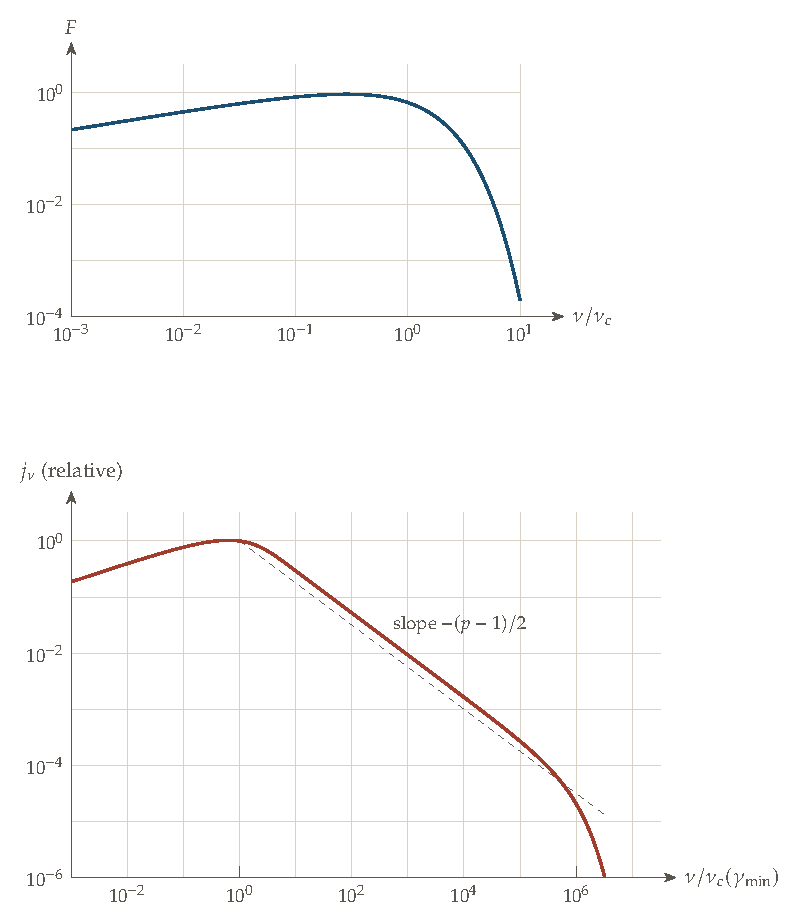
\includegraphics{fig_ch15_sync_spectrum.pdf}
	\caption{Top, the synchrotron spectrum $F(\nu/\nu_c)$ of one electron. Bottom, the spectrum of electrons with $n(\gamma_L)\propto\gamma_L^{-2.5}$ between $\gamma_{\min}$ and $1000\,\gamma_{\min}$, against $\nu/\nu_c(\gamma_{\min})$. Ticks on the frequency axis mark $\nu_c(\gamma_{\min})$ and $\nu_c(\gamma_{\max})$. The dashed line has slope $-0.75$. Computed with \texttt{code/ch15/01\_synchrotron.py}.}
	\label{fp:fig:sync}
\end{figure}

Most radio galaxies have $\alpha\approx0.7$ to $0.8$ in $j_\nu\propto\nu^{-\alpha}$, so their electrons have $p\approx2.4$ to $2.6$. The radio spectrum of the Crab is flatter, $\alpha\approx0.3$, so $p\approx1.6$ there. Where the fastest electrons cool before they escape, the balance of supply and loss (P4) steepens the spectrum. Electrons supplied at a rate $\propto\gamma_L^{-p}$ each survive a time $t_{\rm sync}\propto1/\gamma_L$, so the number present goes as $\gamma_L^{-(p+1)}$, and above that energy $\alpha$ is larger by $\tfrac12$. The frequency of the break gives the age of a radio source. Synchrotron light is also linearly polarised, across the direction of the field projected on the sky, so maps of its polarisation are maps of cosmic magnetic fields. The strong polarisation of the Crab's optical light is what identified it as synchrotron light.

% ==============================================================================
\section{Compton and Inverse Compton Scattering}
\label{fp:sec:compton}

A free electron scatters light with the Thomson cross-section, Eq.~\eqref{eq:thomson_cross_section}, and Table~\ref{tab:scattering_regimes} listed Compton and inverse Compton scattering among the processes that change the photon's energy.

The Thomson result assumes that the electron stays where it is and that the photon leaves with the energy it came with. A hard X-ray photon knocks the electron back. A fast electron throws the photon forward. We need to know how much energy changes hands, and what many such exchanges do to a spectrum.

Think of a tennis ball. Thrown at a fixed wall, it comes back at the speed it arrived. Thrown at a racket swinging toward it, it comes back much faster. To find how much faster, the easiest way is to stand on the racket. There the racket is a wall, the ball bounces back at its arrival speed, and we then add the racket's motion back.

A photon meeting an electron is the ball. If the electron is at rest, a hard photon gives it a kick and loses energy, the Compton effect. If the electron moves fast, the photon in the electron's frame is blue-shifted by about $\gamma_L$, bounces as in Thomson scattering, and is blue-shifted by another $\gamma_L$ on the way back to the lab. The idea is to do the scattering in the electron's frame, where it is plain Thomson scattering, and to carry the photon there and back with the boost matrix of Eq.~\eqref{fp:eq:boost}.

In numbers, a photon of the microwave background, with a mean energy of $6.3\times10^{-4}\,\mathrm{eV}$, meeting an electron with $\gamma_L=10^4$ comes out on average at $85\,\mathrm{keV}$, a hard X-ray.

The picture is a slow photon struck head on and sent back along the electron's path.

The same exchange is the gravity assist of Chapter~\ref{ch:twobody}. In the planet's frame a spacecraft leaves at its arrival speed, and in the Sun's frame it has gained the planet's motion. Inverse Compton scattering makes the X-rays of radio lobes, the gamma rays of pulsar nebulae and blazars, and the X-ray glow of the hot coronae above accretion disks. It uses P1 (conservation of energy and momentum), the boost matrices, P3 for thermal electrons and P5 for the random walk of a photon's energy over many scatterings. It gives the Compton shift, the energy gain and power of inverse Compton scattering, the Compton $y$ parameter and the Sunyaev–Zel'dovich effect.

\paragraph{The Compton shift.} A photon of frequency $\nu$ meets an electron at rest and leaves at angle $\psi$ with frequency $\nu_1$. Write four-momenta as (energy over $c$, momentum), with the dot product $A\cdot B=A^0B^0-\vec A\cdot\vec B$. The photon has $k=(h\nu/c)(1,\hat n)$ before and $k_1=(h\nu_1/c)(1,\hat n_1)$ after, and the electron has $q=(m_ec,\vec0)$ before and $q_1$ after. Conservation (P1) is $q+k=q_1+k_1$.
\begin{align}
	m_e^2c^2
	&\eqby{1} q_1\cdot q_1=(q+k-k_1)\cdot(q+k-k_1) \nonumber\\
	&\eqby{2} m_e^2c^2+2\,q\cdot k-2\,q\cdot k_1-2\,k\cdot k_1 \nonumber\\
	\implies\quad m_eh(\nu-\nu_1)
	&\eqby{3} \frac{h^2\nu\nu_1}{c^2}\,(1-\cos\psi) \nonumber\\
	\implies\quad \frac{c}{\nu_1}-\frac{c}{\nu}
	&\eqby{4} \frac{h}{m_ec}\,(1-\cos\psi) .
\end{align}
\begin{explain}
	\item The electron's mass is the same before and after. Conservation gives $q_1$.
	\item Expand. $q\cdot q=m_e^2c^2$, and $k\cdot k=k_1\cdot k_1=0$ for photons.
	\item $q\cdot k=m_eh\nu$, $q\cdot k_1=m_eh\nu_1$, and $k\cdot k_1=(h^2\nu\nu_1/c^2)(1-\hat n\cdot\hat n_1)$ with $\hat n\cdot\hat n_1=\cos\psi$.
	\item Divide by $m_eh\nu\nu_1/c$.
\end{explain}
\begin{equation}
	\boxed{\lambda_1-\lambda=\lambda_C\,(1-\cos\psi),\qquad h\nu_1=\frac{h\nu}{1+(h\nu/m_ec^2)(1-\cos\psi)},}
	\label{fp:eq:compton_shift}
\end{equation}
with the Compton wavelength $\lambda_C=h/(m_ec)=2.43\times10^{-12}\,\mathrm m$ and $m_ec^2=511\,\mathrm{keV}$. The shift in wavelength does not depend on the wavelength. It matters only when $\lambda$ is not much longer than $\lambda_C$, that is when $h\nu$ approaches $m_ec^2$. For $h\nu\ll m_ec^2$ the photon keeps its energy, the Thomson limit. A $10\,\mathrm{keV}$ X-ray scattered by cold electrons loses about $2\%$ of its energy each time.

\paragraph{Inverse Compton, there and back.} Now let the electron move with $\gamma_L$ along $x$, and let a photon of frequency $\nu$ arrive at angle $\theta$ to the electron's velocity. Into the electron's frame, with $\Lambda(-\beta)$,
\begin{align}
	\frac{h\nu'}{c}\begin{pmatrix}1\\ \cos\theta'\\ \sin\theta'\end{pmatrix}
	&\eqby{1} \begin{pmatrix}\gamma_L&-\gamma_L\beta&0\\-\gamma_L\beta&\gamma_L&0\\0&0&1\end{pmatrix}\frac{h\nu}{c}\begin{pmatrix}1\\ \cos\theta\\ \sin\theta\end{pmatrix}
	=\frac{h\nu}{c}\begin{pmatrix}\gamma_L(1-\beta\cos\theta)\\ \gamma_L(\cos\theta-\beta)\\ \sin\theta\end{pmatrix} \nonumber\\
	\implies\quad \nu'
	&\eqby{2} \gamma_L(1-\beta\cos\theta)\,\nu .
\end{align}
\begin{explain}
	\item The inverse boost of Eq.~\eqref{fp:eq:boost} applied to the photon's four-momentum.
	\item The first row.
\end{explain}
If $h\nu'\ll m_ec^2$, the scattering in the electron's frame is Thomson scattering. The photon keeps the frequency $\nu'$ and leaves at some angle $\theta'_1$. Back to the lab, with $\Lambda(\beta)$, the first row of Eq.~\eqref{fp:eq:beaming} gives
\begin{equation}
	\boxed{\nu_1=\gamma_L(1+\beta\cos\theta'_1)\,\nu'=\gamma_L^2\,(1-\beta\cos\theta)(1+\beta\cos\theta'_1)\,\nu .}
	\label{fp:eq:ic_boost}
\end{equation}
A photon met head on, $\theta=\pi$, and sent back forward, $\theta'_1=0$, gains the most, $\nu_1=\gamma_L^2(1+\beta)^2\nu\approx4\gamma_L^2\nu$. One factor $\gamma_L$ comes from each boost. The condition $h\nu'\approx\gamma_Lh\nu\ll m_ec^2$ must hold in the electron's frame. When it fails, the recoil of Eq.~\eqref{fp:eq:compton_shift} takes over in that frame, and the photon can gain at most about the electron's own energy $\gamma_Lm_ec^2$.

\paragraph{The power.} Let the electron move through photons of energy density $u_{\rm rad}$, coming equally from all directions. Photons from angle $\theta$ meet the electron at the closing speed $c(1-\beta\cos\theta)$, so a fraction $d\Omega/4\pi$ of them, carrying energy density $u_{\rm rad}\,d\Omega/4\pi$, is scattered at the rate $\sigma_Tc(1-\beta\cos\theta)$ per unit of photon density. The Thomson pattern sends as much forward as backward in the electron's frame, so $\cos\theta'_1$ averages to zero in Eq.~\eqref{fp:eq:ic_boost}. The power that leaves in scattered photons, minus the power those photons brought in, is
\begin{align}
	\mathcal P
	&\eqby{1} \sigma_Tc\int\frac{d\Omega}{4\pi}\,u_{\rm rad}\,(1-\beta\cos\theta)\Big[\gamma_L^2(1-\beta\cos\theta)-1\Big] \nonumber\\
	&\eqby{2} \sigma_Tc\,u_{\rm rad}\Big[\gamma_L^2\Big(1+\frac{\beta^2}{3}\Big)-1\Big] \nonumber\\
	&\eqby{3} \sigma_Tc\,u_{\rm rad}\Big[\gamma_L^2\beta^2+\frac{\gamma_L^2\beta^2}{3}\Big] .
\end{align}
\begin{explain}
	\item Rate of scattering times the energy gained, which is $\gamma_L^2(1-\beta\cos\theta)$ times the arriving energy by Eq.~\eqref{fp:eq:ic_boost}, minus the arriving energy.
	\item $\int(1-\beta\cos\theta)^2\,d\Omega/4\pi=1+\beta^2/3$ and $\int(1-\beta\cos\theta)\,d\Omega/4\pi=1$.
	\item $\gamma_L^2-1=\gamma_L^2\beta^2$.
\end{explain}
\begin{equation}
	\boxed{\mathcal P=\frac43\,\sigma_Tc\,\gamma_L^2\beta^2\,u_{\rm rad} .}
	\label{fp:eq:ic_power}
\end{equation}
This has the form of the synchrotron power, Eq.~\eqref{fp:eq:sync_power}, with the energy density of light in place of that of the field. A fast electron loses energy to the two in the ratio $u_{\rm rad}/u_B$. Since photons are scattered at the rate $\sigma_Tc\,u_{\rm rad}/\avg{h\nu}$, the mean energy of a scattered photon is $\tfrac43\gamma_L^2\avg{h\nu}$.

The microwave background fills all space with $u_{\rm rad}=a_{\rm rad}T^4=4.2\times10^{-14}\,\mathrm{J\,m^{-3}}$, using Eq.~\eqref{pr:eq:photon_gas} at $2.725\,\mathrm K$. That equals the energy density of a field of $0.32\,\mathrm{nT}$. In radio lobes, with fields of order $1\,\mathrm{nT}$, scattering the background costs the electrons a tenth or more of what synchrotron light costs them, and the scattered photons come out as X-rays. In the Crab the electrons scatter their own synchrotron photons up to gamma rays.

\paragraph{Many scatterings in hot gas.} Now let the electrons be thermal, with $\beta\ll1$, and let the photons have $h\nu\ll k_BT$. Two numbers describe one scattering. The mean fractional gain follows from Eq.~\eqref{fp:eq:ic_power} divided by the scattering rate, with $\avg{\gamma_L^2\beta^2}\approx\avg{v^2}/c^2=3k_BT/m_ec^2$ from the Maxwell distribution (P3). The spread follows from Eq.~\eqref{fp:eq:ic_boost} at first order in $\beta$, $\Delta\nu/\nu=\beta(\cos\theta'_1-\cos\theta)$, where the incoming and outgoing directions are unrelated to the electron's velocity and each has $\avg{\cos^2}=\tfrac13$,
\begin{equation}
	\avg{\frac{\Delta\nu}{\nu}}=\frac43\cdot\frac{3k_BT}{m_ec^2}=\frac{4k_BT}{m_ec^2},\qquad
	\avg{\Big(\frac{\Delta\nu}{\nu}\Big)^2}=\frac{3k_BT}{m_ec^2}\Big(\frac13+\frac13\Big)=\frac{2k_BT}{m_ec^2} .
	\label{fp:eq:ic_moments}
\end{equation}
The recoil of Eq.~\eqref{fp:eq:compton_shift}, a loss of $h\nu/m_ec^2$, is negligible for $h\nu\ll k_BT$. Each scattering counts as a step of size $k_BT/m_ec^2$, so the effect of a cloud is measured by the \textbf{Compton $y$ parameter},
\begin{equation}
	\boxed{y=\int\frac{k_BT}{m_ec^2}\,n_e\sigma_T\,dl ,}
	\label{fp:eq:compton_y}
\end{equation}
the number of scatterings times $k_BT/m_ec^2$. A thin cloud scatters a photon about $\tau=\int n_e\sigma_Tdl$ times, and a thick one about $\tau^2$ times by the random walk of Eq.~\eqref{pr:eq:walk_time} (P5).

\paragraph{The random walk in frequency.} Each photon takes a random walk in $x=h\nu/k_BT_\gamma$, where $T_\gamma$ is any fixed reference temperature, with a drift. Let $N(x)\,dx$ be the number of photons in $dx$. Per unit $y$, Eq.~\eqref{fp:eq:ic_moments} gives a mean step $4x$ and a mean square step $2x^2$. Photons drift up with the flux $4xN$, and they spread by a random walk (P5), as in Eq.~\eqref{pr:eq:fick} but with a step that depends on $x$. The number of photons is conserved (P1), so $N$ obeys a continuity equation. With $N=x^2f$, where $f$ is the photon occupation number of Section~\ref{pr:sec:p3},
\begin{align}
	\pdv{N}{y}
	&\eqby{1} -\pdv{x}\Big[4xN-\frac12\pdv{x}\big(2x^2N\big)\Big] \nonumber\\
	&\eqby{2} -\pdv{x}\Big[4x^3f-\pdv{x}\big(x^4f\big)\Big] \nonumber\\
	&\eqby{3} \pdv{x}\Big(x^4\pdv{f}{x}\Big) .
\end{align}
\begin{explain}
	\item Continuity in $x$ (P1). The flux is the drift plus the random walk. For the walk, let a photon at $x$ step up or down by $\delta(x)$ with equal chances. Photons within $\delta$ below a point cross it upward with chance $\tfrac12$, and those within $\delta$ above cross downward, so the net flux is $\tfrac12N\delta$ half a step below minus $\tfrac12N\delta$ half a step above, $-\tfrac12\,\partial(\delta^2N)/\partial x$. Per unit $y$, $\delta^2$ averages to $2x^2$.
	\item $N=x^2f$.
	\item $\partial(x^4f)/\partial x=4x^3f+x^4\,\partial f/\partial x$, and the $4x^3f$ terms cancel.
\end{explain}
\begin{equation}
	\boxed{\pdv{\big(x^2f\big)}{y}=\pdv{x}\Big(x^4\pdv{f}{x}\Big).}
	\label{fp:eq:kompaneets}
\end{equation}
This is the Kompaneets equation, in the limit where recoil can be neglected. Multiplying by $x$ and integrating over all $x$ by parts twice gives $d\avg{x}/dy=4\avg{x}$, so the mean photon energy grows as $e^{4y}$. Where $y\gtrsim1$, photons from a cool source are lifted into a power law of X-rays, which is how the hot coronae above accretion disks make their X-rays.

\paragraph{The Sunyaev–Zel'dovich effect.} Light of the microwave background crossing the hot gas of a cluster has $y\ll1$. Take $T_\gamma$ to be its temperature, so before the cluster $f_0=1/(e^x-1)$. To first order in $y$, Eq.~\eqref{fp:eq:kompaneets} gives
\begin{align}
	\frac{\Delta f}{f_0}
	&\eqby{1} \frac{y}{x^2f_0}\,\dv{x}\Big(x^4\dv{f_0}{x}\Big) \nonumber\\
	&\eqby{2} y\,\frac{xe^x}{e^x-1}\Big(x\,\frac{e^x+1}{e^x-1}-4\Big)
	\ \xrightarrow{\ x\ll1\ }\ -2y .
	\label{fp:eq:sz}
\end{align}
\begin{explain}
	\item Integrate Eq.~\eqref{fp:eq:kompaneets} across the cluster with the right-hand side evaluated on $f_0$.
	\item $df_0/dx=-e^x/(e^x-1)^2$, differentiated once more. For $x\ll1$ the first factor tends to $1$ and the bracket to $2-4$.
\end{explain}
At low frequencies, where the intensity is proportional to the temperature, the background seen through the cluster looks colder,
\[
\boxed{\frac{\Delta T}{T_{\rm CMB}}=-2y\qquad(h\nu\ll k_BT_{\rm CMB}).}
\]
Photons are moved up in frequency, and none is lost, so the dip at low frequency is paid for by an excess at high frequency. The change is zero at $x=3.83$, $217\,\mathrm{GHz}$ (Figure~\ref{fp:fig:sz}). A cluster with $n_e=10^3\,\mathrm{m^{-3}}$ and $k_BT=6\,\mathrm{keV}$ across $1\,\mathrm{Mpc}$ has $\tau=2.1\times10^{-3}$, $k_BT/m_ec^2=0.012$ and $y=2.4\times10^{-5}$, so the background dims by $130\,\mu\mathrm K$. The dip is a fixed fraction of the background itself, so it does not fade with the distance of the cluster (P6). Surveys find clusters by it out to great distances.

\begin{figure}[htbp]
	\centering
	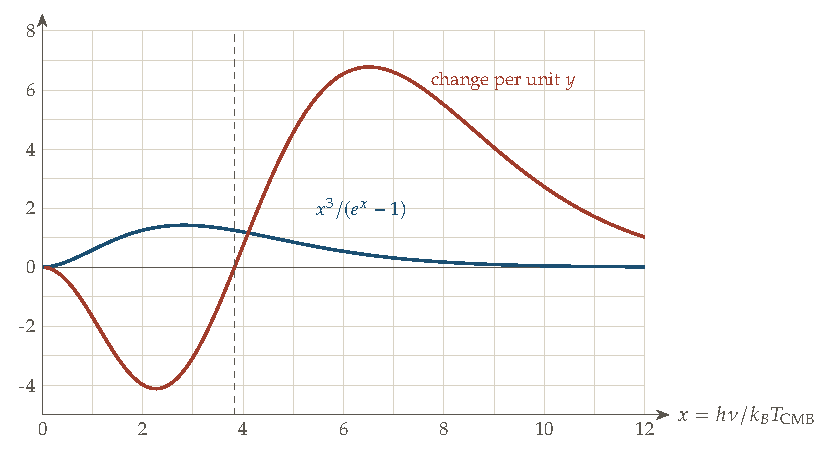
\includegraphics{fig_ch15_sz_distortion.pdf}
	\caption{The microwave background intensity shape $x^3/(e^x-1)$, and its change per unit $y$ after crossing hot gas, $x^4e^x(e^x-1)^{-2}[x(e^x+1)/(e^x-1)-4]$, both in units of $2(k_BT_{\rm CMB})^3/(hc)^2$. The dashed line marks $x=3.83$.}
	\label{fp:fig:sz}
\end{figure}

% ==============================================================================
\section{Accretion and Active Galaxies}
\label{fp:sec:accretion}

The compactness $GM/(Rc^2)$ measures how deep the gravitational well at the surface of a body is, against $c^2$ (Section~\ref{cs:sec:compactness}). The Eddington luminosity caps how brightly a mass $M$ can shine (Eq.~\eqref{rad:eq:eddington}).

A quasar shines at about $10^{40}\,\mathrm W$, a thousand times a large galaxy of $10^{10}$ to $10^{11}$ Suns, and it changes in brightness within days, so the light comes from a region a few light-days across. Nuclear burning releases only $0.7\%$ of the rest mass of its fuel (Section~\ref{st:sec:eos}). The fuel needed by nuclear burning would not fit in so small a region, and it would take too long to burn. Something more powerful is at work.

Think of water flowing over a dam. Each kilogram that falls turns the turbines with an energy set by the height of the fall. A taller dam gives more energy from each kilogram, and the power is that energy times the kilograms per second.

Gas falling onto a compact object falls down a very deep well. Each kilogram releases $GM/R$, which is $c^2$ times the compactness. The idea is that the share of rest mass released by accretion equals the compactness, up to tens of percent, and that the gas, spiralling in through a disk, radiates the energy locally as heat (P1, P4).

In numbers, matter falling onto a neutron star releases $0.17$ of its rest mass, $25$ times more per kilogram than burning hydrogen. A quasar shining at $10^{40}\,\mathrm W$ with an efficiency of $0.1$ swallows $1.1\times10^{24}\,\mathrm{kg\,s^{-1}}$, $18$ solar masses a year.

The picture is gas spiralling slowly inward in a thin, flat disk, hotter toward the centre, with narrow jets leaving along the axis.

The same process powers X-ray binaries, the outbursts of white dwarfs in binaries, the disks round young stars, and the nuclei of active galaxies. It uses P1 for energy and for angular momentum, P2, P4 for the local balance of heating and cooling, and P6 for light-travel times. It gives the luminosity and efficiency of accretion, black-hole masses, the temperature and spectrum of a thin disk, and the apparent speeds of jets.

\paragraph{Accretion luminosity.} Matter falling from far away onto the surface of a body of mass $M$ and radius $R$, at the rate $\dot M$, loses the potential energy $GM/R$ per unit mass, which ends up as heat and light (P1),
\begin{equation}
	\boxed{L=\frac{GM\dot M}{R},\qquad \eta\equiv\frac{L}{\dot Mc^2}=\frac{GM}{Rc^2} .}
	\label{fp:eq:accretion_L}
\end{equation}
The \textbf{efficiency} $\eta$ is the compactness of Table~\ref{cs:tab:compactness}, $2.6\times10^{-4}$ for a white dwarf like Sirius B and $0.17$ for a neutron star. A black hole has no surface. Gas radiates while it spirals down to the last stable circular orbit, which general relativity puts at $6GM/c^2$ for a black hole without spin. The efficiency is then $1-\sqrt{8/9}=0.057$, and it rises to $0.42$ for the fastest spin allowed. These two numbers are quoted from general relativity. The Newtonian estimate, half of $GM/R$ at $R=6GM/c^2$ (the half is explained below), gives $1/12=0.083$.

\paragraph{The Eddington limit and black-hole masses.} Light from the infalling gas pushes it back. By Eq.~\eqref{rad:eq:eddington} a steady source of mass $M$ shines at most at $1.26\times10^{31}\,\mathrm W\,(M/M_\odot)$. A quasar at $10^{40}\,\mathrm W$ therefore holds at least $8\times10^8\,M_\odot$ (Problem~\ref{rad:prob:eddington}). A change in brightness within a day limits its size to the distance light travels in a day, $2.6\times10^{13}\,\mathrm m$, since the far side of a larger source would not hear in time that it should brighten (P6). The Schwarzschild radius of $10^9\,M_\odot$ is $3\times10^{12}\,\mathrm m$. So the mass is packed into a few tens of Schwarzschild radii at most, and only a black hole fits.

\paragraph{The thin disk, angular momentum.} Gas does not fall straight in. It has angular momentum, and it settles into a thin disk where each ring circles at the Kepler angular velocity $\sqrt{GM/r^3}$, with angular momentum $\sqrt{GMr}$ per unit mass. A ring can move inward only by handing angular momentum outward, which friction between neighbouring rings does. Let $\mathcal T(r)$ be the torque that the gas inside $r$ exerts on the gas outside. In a steady disk the angular momentum carried inward through $r$ by the gas, minus that carried outward by the torque, is the same at every radius (P1). At the inner edge $R_{\rm in}$ the gas falls freely into the hole, so the torque there is zero.
\begin{align}
	\dot M\sqrt{GMr}-\mathcal T(r)
	&\eqby{1} \dot M\sqrt{GMR_{\rm in}}-0 \nonumber\\
	\implies\quad \mathcal T(r)
	&= \dot M\sqrt{GM}\,\big(\sqrt r-\sqrt{R_{\rm in}}\big) .
	\label{fp:eq:torque}
\end{align}
\begin{explain}
	\item The constant evaluated at the inner edge, where $\mathcal T=0$.
\end{explain}

\paragraph{The thin disk, energy.} The energy flowing outward through radius $r$ has two parts. The gas, moving inward, carries its orbital energy $-GM/2r$ per unit mass, which is an outward flow of $\dot MGM/2r$. The torque does work on the outer gas at the rate $\mathcal T\sqrt{GM/r^3}$. What the ring between $r$ and $r+dr$ takes from this flow, it radiates (P1). Both faces radiate as blackbodies at the local temperature $T(r)$ (P4, Eq.~\eqref{eq:surface_flux_sb}).
\begin{align}
	2\cdot2\pi r\,dr\;\sigma_{\rm SB}T^4
	&\eqby{1} -\dv{r}\Big[\frac{GM\dot M}{2r}+\mathcal T\sqrt{\frac{GM}{r^3}}\,\Big]dr \nonumber\\
	&\eqby{2} -GM\dot M\,\dv{r}\Big[\frac{1}{2r}+\frac1r-\frac{\sqrt{R_{\rm in}}}{r^{3/2}}\Big]dr \nonumber\\
	&\eqby{3} GM\dot M\Big[\frac{3}{2r^2}-\frac{3\sqrt{R_{\rm in}}}{2r^{5/2}}\Big]dr
	= \frac{3GM\dot M}{2r^2}\Big(1-\sqrt{\frac{R_{\rm in}}{r}}\Big)dr .
\end{align}
\begin{explain}
	\item Radiation from the two faces of the ring equals the energy flow into it from inside minus the flow out of it.
	\item The torque \eqref{fp:eq:torque}, so $\mathcal T\sqrt{GM/r^3}=GM\dot M\big(r^{-1}-\sqrt{R_{\rm in}}\,r^{-3/2}\big)$.
	\item Differentiate term by term.
\end{explain}
\begin{equation}
	\boxed{\sigma_{\rm SB}T^4=\frac{3GM\dot M}{8\pi r^3}\Big(1-\sqrt{\frac{R_{\rm in}}{r}}\Big),\qquad T\propto r^{-3/4}\ \text{for }r\gg R_{\rm in}.}
	\label{fp:eq:disk_T}
\end{equation}
The mass and the accretion rate set the temperature together, as $M\dot M$. Far out, a ring radiates three times the orbital energy that its own gas gives up. The extra two thirds is energy carried outward by the torque from the rings inside.

As a check by energy alone, the whole disk radiates
\[
\int_{R_{\rm in}}^\infty\frac{3GM\dot M}{2r^2}\Big(1-\sqrt{\frac{R_{\rm in}}{r}}\Big)dr=\frac{GM\dot M}{2R_{\rm in}},
\]
half of the energy $GM\dot M/R_{\rm in}$ released by the fall. The other half is the orbital kinetic energy the gas still has at $R_{\rm in}$, as the virial theorem requires for a circular orbit (Section~\ref{sg:sec:virial}). On a star it is released where the gas meets the surface, and a black hole swallows it.

Writing $T_*=(3GM\dot M/8\pi\sigma_{\rm SB}R_{\rm in}^3)^{1/4}$, the temperature is $T=T_*(R_{\rm in}/r)^{3/4}(1-\sqrt{R_{\rm in}/r})^{1/4}$. It peaks at $r=\tfrac{49}{36}R_{\rm in}$, where $T=0.488\,T_*$ (Figure~\ref{fp:fig:disk}). For a black hole of $10^8\,M_\odot$ fed $1\,M_\odot$ a year, with $R_{\rm in}=6GM/c^2$, the hottest ring is at $1.1\times10^5\,\mathrm K$ and the disk shines in the ultraviolet with $4.7\times10^{38}\,\mathrm W$. For a black hole of $10\,M_\odot$ fed $10^{-8}\,M_\odot$ a year it is at $3.5\times10^6\,\mathrm K$, $k_BT=0.30\,\mathrm{keV}$, in X-rays. With $R_{\rm in}\propto M$, $T_*\propto(\dot M/M^2)^{1/4}$, and at a fixed fraction of the Eddington limit $\dot M\propto M$, so $T_*\propto M^{-1/4}$. Small black holes have hotter disks.

\begin{figure}[htbp]
	\centering
	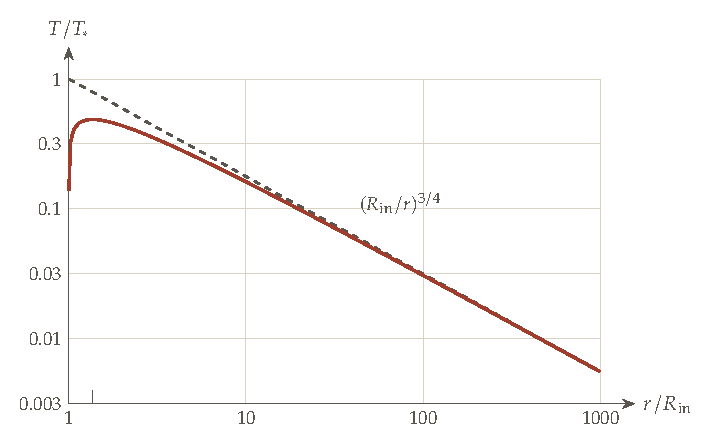
\includegraphics{fig_ch15_disk_temperature.pdf}
	\caption{Temperature of a thin accretion disk, $T/T_*=(R_{\rm in}/r)^{3/4}(1-\sqrt{R_{\rm in}/r})^{1/4}$, against radius, with the power law $(R_{\rm in}/r)^{3/4}$ dashed. The tick marks $r=\tfrac{49}{36}R_{\rm in}$.}
	\label{fp:fig:disk}
\end{figure}

\paragraph{The spectrum of the disk.} By Eq.~\eqref{ph:eq:flux_pi_B}, each face of a ring sends out the flux $\pi B_\nu(T(r))$. Far from the inner edge, $T=T_*(R_{\rm in}/r)^{3/4}$. To add up the rings at a frequency $\nu$, change the variable from $r$ to $u=h\nu/k_BT(r)=(h\nu/k_BT_*)(r/R_{\rm in})^{3/4}$, so that $r=R_{\rm in}(uk_BT_*/h\nu)^{4/3}$.
\begin{align}
	L_\nu
	&\eqby{1} \int 2\cdot2\pi r\;\pi B_\nu\big(T(r)\big)\,dr \nonumber\\
	&\eqby{2} 4\pi^2\,\frac{2h\nu^3}{c^2}\int\frac{r\,dr}{e^{u}-1} \nonumber\\
	&\eqby{3} 4\pi^2\,\frac{2h\nu^3}{c^2}\,\frac43\,R_{\rm in}^2\left(\frac{k_BT_*}{h\nu}\right)^{8/3}\int_0^\infty\frac{u^{5/3}\,du}{e^u-1}
	\ \propto\ \nu^{1/3} .
	\label{fp:eq:disk_spectrum}
\end{align}
\begin{explain}
	\item Two faces of each ring of area $2\pi r\,dr$.
	\item The Planck function \eqref{pr:eq:planck} with $h\nu/k_BT(r)=u$.
	\item $r\,dr=\tfrac43R_{\rm in}^2(k_BT_*/h\nu)^{8/3}u^{5/3}du$. For $k_BT(\text{outer edge})\ll h\nu\ll k_BT_*$ the limits of $u$ are $0$ and $\infty$, and the integral is the number $\Gamma(\tfrac83)\zeta(\tfrac83)=1.93$.
\end{explain}
Between the temperatures of the outer and inner edges a disk is neither a blackbody nor the power law of fast electrons. It is a blackbody stretched over many temperatures, $L_\nu\propto\nu^{1/3}$, cut off at the frequency of its hottest ring. In quasars this hump appears in the ultraviolet.

\paragraph{Faster than light.} Jets from active nuclei carry blobs of radio-emitting plasma outward, and radio interferometers (Chapter~\ref{ch:resolution}) follow them across the sky. Many seem to move faster than light. Let a blob leave the core at $t=0$ with speed $\beta c$ at angle $\theta$ to the line of sight. At time $t$ it has moved $\beta ct\cos\theta$ toward us and $\beta ct\sin\theta$ across the sky. Its light set out from a point $\beta ct\cos\theta$ nearer to us, so the light from the two moments arrives separated by less than $t$ (P6).
\begin{align}
	\Delta t_{\rm obs}
	&\eqby{1} t-\frac{\beta ct\cos\theta}{c}=t\,(1-\beta\cos\theta) \nonumber\\
	\implies\quad \beta_{\rm app}
	&\eqby{2} \frac{\beta ct\sin\theta}{c\,\Delta t_{\rm obs}}=\frac{\beta\sin\theta}{1-\beta\cos\theta} .
\end{align}
\begin{explain}
	\item The time between emissions minus the head start of the later light.
	\item The apparent speed across the sky, in units of $c$, is the sideways distance over the observed time.
\end{explain}
\begin{equation}
	\boxed{\beta_{\rm app}=\frac{\beta\sin\theta}{1-\beta\cos\theta}.}
	\label{fp:eq:superluminal}
\end{equation}
Its derivative with respect to $\theta$ is $\beta(\cos\theta-\beta)/(1-\beta\cos\theta)^2$, which is zero at $\cos\theta=\beta$. There $\sin\theta=1/\gamma_L$ and $\beta_{\rm app}=\beta\gamma_L$, which exceeds $1$ for $\beta>1/\sqrt2$ (Figure~\ref{fp:fig:superluminal}). Nothing moves faster than light. The blob nearly keeps up with its own light, so a long time of travel is squeezed into a short time of observation, the same squeezing as in the synchrotron flash. Since $\beta_{\rm app}\le\beta\gamma_L<\gamma_L$, a measured apparent speed gives a lower limit on the Lorentz factor of the jet. The jet of M87 shows features moving at about $6c$, so its Lorentz factor is at least $6$ (Problem~\ref{fp:prob:m87}). By Eq.~\eqref{fp:eq:beaming}, light from the approaching jet is raised in frequency and thrown forward, and light from the receding jet is lowered and thrown away from us. That is why most jets look one-sided.

\begin{figure}[htbp]
	\centering
	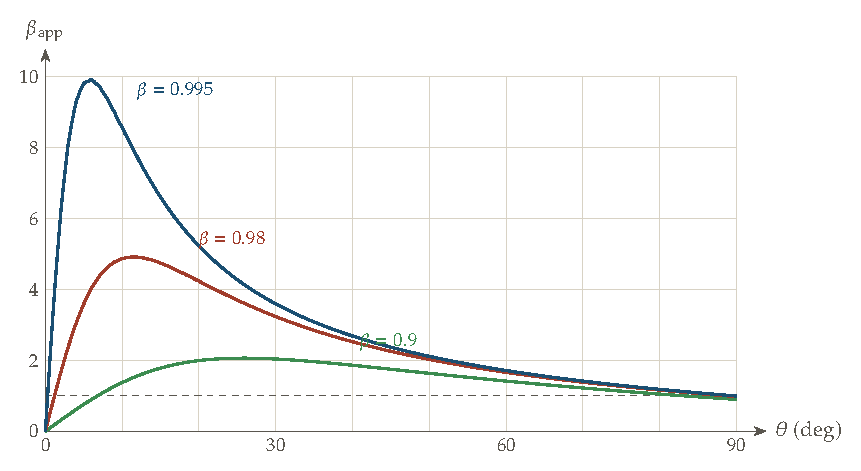
\includegraphics{fig_ch15_superluminal.pdf}
	\caption{Apparent speed across the sky, $\beta_{\rm app}=\beta\sin\theta/(1-\beta\cos\theta)$, against the angle $\theta$ between the motion and the line of sight, for $\beta=0.9$, $0.98$ and $0.995$. The dashed line marks $\beta_{\rm app}=1$.}
	\label{fp:fig:superluminal}
\end{figure}

\paragraph{Active galaxies.} A normal galaxy (Chapter~\ref{ch:galaxies}) shines with the light of its stars. In an active galaxy a nucleus of a few light-days adds light from a hot disk, from bremsstrahlung, from synchrotron light and from inverse Compton scattering. The accretion disk gives the ultraviolet hump of Eq.~\eqref{fp:eq:disk_spectrum}. Hot electrons above the disk scatter its photons up into X-rays with $y\gtrsim1$. Jets and the lobes they feed shine by synchrotron light in the radio, with spectra like Eq.~\eqref{fp:eq:sync_index}, and by inverse Compton scattering in X-rays and gamma rays. Where a jet points almost at us, its light is beamed and boosted, and the source, a blazar, can change within hours. Seyfert galaxies, quasars, radio galaxies and blazars differ mainly in luminosity and in the angle from which we see them. All of them draw their power from gas falling into a black hole of $10^6$ to $10^{10}\,M_\odot$, with the efficiency of Eq.~\eqref{fp:eq:accretion_L}.

% ==============================================================================
\section{Problem Set: Radiation from Hot and Fast Particles}

\subsection{Problem 1: X-rays From a Cluster of Galaxies}
\label{fp:prob:cluster}

\textbf{Problem Statement}: A cluster of galaxies holds ionised hydrogen with $n_e=n_i=10^3\,\mathrm{m^{-3}}$ at $T=7\times10^7\,\mathrm K$, filling a sphere of radius $1\,\mathrm{Mpc}=3.09\times10^{22}\,\mathrm m$. Take $\bar g=1$. Find (a) the power radiated per unit volume, (b) the X-ray luminosity, (c) the cooling time, compared with the age of the universe, $1.4\times10^{10}$ years, and (d) the photon energy at which the spectrum has fallen to $1/e$ of its low-frequency value.

\textbf{Essential Ideas}:
\begin{itemize}
	\item The cooling rate $1.4\times10^{-40}\,n_en_i\sqrt T\ \mathrm{W\,m^{-3}}$, Eq.~\eqref{fp:eq:brems_total}.
	\item The thermal energy $3nk_BT$ per unit volume, and the spectrum $\propto e^{-h\nu/k_BT}$ of Eq.~\eqref{fp:eq:brems_jnu}.
\end{itemize}

\textbf{Detailed Solutions}:
\begin{enumerate}[label=(\alph*)]
	\item \textbf{Power per volume}. $1.4\times10^{-40}\times10^6\times\sqrt{7\times10^7}$.
	\[
	\boxed{1.2\times10^{-30}\,\mathrm{W\,m^{-3}}.}
	\]
	\item \textbf{Luminosity}. The volume is $\tfrac43\pi(3.09\times10^{22})^3=1.2\times10^{68}\,\mathrm{m^3}$.
	\[
	\boxed{L_X\simeq1.5\times10^{38}\,\mathrm W.}
	\]
	\item \textbf{Cooling time}. $3nk_BT=2.9\times10^{-12}\,\mathrm{J\,m^{-3}}$, divided by the power per volume.
	\[
	\boxed{t_{\rm cool}\simeq2.4\times10^{18}\,\mathrm s\simeq8\times10^{10}\ \text{years}.}
	\]
	This is more than five times the age of the universe, so the gas has kept its heat since the cluster formed.
	\item \textbf{Cut-off}. The spectrum falls by $e$ at $h\nu=k_BT$.
	\[
	\boxed{h\nu=6.0\,\mathrm{keV},\qquad \nu=1.5\times10^{18}\,\mathrm{Hz}.}
	\]
	Fitting the turn-down of a measured X-ray spectrum gives the gas temperature, and with Eq.~\eqref{sg:eq:hse} the mass of the cluster.
\end{enumerate}

\subsection{Problem 2: Electrons in a Radio Lobe}
\label{fp:prob:lobe}

\textbf{Problem Statement}: A radio lobe has a field $B=1\,\mathrm{nT}$ and is observed at $1.4\,\mathrm{GHz}$. Its spectrum is $j_\nu\propto\nu^{-0.75}$. Find (a) the Lorentz factor of the electrons that radiate at $1.4\,\mathrm{GHz}$, taking $\nu=\tfrac32\gamma_L^2\nu_g$, (b) their synchrotron lifetime, (c) the index $p$ of the electrons, and (d) how much the scattering of the microwave background ($u_{\rm rad}=4.2\times10^{-14}\,\mathrm{J\,m^{-3}}$) shortens their life.

\textbf{Essential Ideas}:
\begin{itemize}
	\item $\nu_g=2.80\times10^{10}\,\mathrm{Hz}\,(B/1\,\mathrm T)$, Eq.~\eqref{fp:eq:gyro}.
	\item $t_{\rm sync}=3m_ec/(4\sigma_T\gamma_Lu_B)$ with $u_B=B^2/2\mu_0$, and the inverse Compton power has $u_{\rm rad}$ in place of $u_B$ (Eq.~\eqref{fp:eq:ic_power}).
	\item $\alpha=(p-1)/2$, Eq.~\eqref{fp:eq:sync_index}.
\end{itemize}

\textbf{Detailed Solutions}:
\begin{enumerate}[label=(\alph*)]
	\item \textbf{Lorentz factor}. $\nu_g=28.0\,\mathrm{Hz}$, so $\gamma_L=\sqrt{1.4\times10^9/(1.5\times28.0)}$.
	\[
	\boxed{\gamma_L\simeq5.8\times10^3,\qquad \gamma_Lm_ec^2\simeq3\,\mathrm{GeV}.}
	\]
	\item \textbf{Lifetime}. $u_B=(10^{-9})^2/(2\times1.26\times10^{-6})=4.0\times10^{-13}\,\mathrm{J\,m^{-3}}$.
	\[
	\boxed{t_{\rm sync}=\frac{3\times9.11\times10^{-31}\times3.00\times10^8}{4\times6.65\times10^{-29}\times5.8\times10^3\times4.0\times10^{-13}}\,\mathrm s\simeq1.3\times10^{15}\,\mathrm s\simeq4\times10^7\ \text{years}.}
	\]
	\item \textbf{Electron index}. $0.75=(p-1)/2$.
	\[
	\boxed{p=2.5.}
	\]
	\item \textbf{Scattering the background}. The two losses add, so the lifetime is $t_{\rm sync}$ divided by $1+u_{\rm rad}/u_B=1+0.105$.
	\[
	\boxed{t\simeq3.8\times10^7\ \text{years}.}
	\]
	Synchrotron losses dominate in this field. In a lobe with a field below $0.32\,\mathrm{nT}$ the scattering of the background would dominate, and the lobe would shine more brightly in X-rays than its radio light suggests.
\end{enumerate}

\subsection{Problem 3: Photons Kicked and Thrown}
\label{fp:prob:compton}

\textbf{Problem Statement}: (a) A gamma ray of $511\,\mathrm{keV}$ is scattered through $90^\circ$ by an electron at rest. What is its energy afterwards? (b) Electrons with $\gamma_L=10^4$ scatter photons of the microwave background, of mean energy $6.3\times10^{-4}\,\mathrm{eV}$. What is the mean energy of the scattered photons, and the largest energy for a photon of that mean energy? (c) Is the Thomson limit valid in (b)? (d) For the cluster of Problem~\ref{fp:prob:cluster}, find $y$ along a path of $1\,\mathrm{Mpc}$ and the dip in the temperature of the background at low frequency ($T_{\rm CMB}=2.725\,\mathrm K$).

\textbf{Essential Ideas}:
\begin{itemize}
	\item $h\nu_1=h\nu/[1+(h\nu/m_ec^2)(1-\cos\psi)]$, Eq.~\eqref{fp:eq:compton_shift}.
	\item Mean gain $\tfrac43\gamma_L^2$ and largest gain $4\gamma_L^2$ (Eqs.~\eqref{fp:eq:ic_boost} and~\eqref{fp:eq:ic_power}), valid while $\gamma_Lh\nu\ll m_ec^2$.
	\item $y=(k_BT/m_ec^2)\,n_e\sigma_TL$ and $\Delta T/T=-2y$, Eqs.~\eqref{fp:eq:compton_y} and~\eqref{fp:eq:sz}.
\end{itemize}

\textbf{Detailed Solutions}:
\begin{enumerate}[label=(\alph*)]
	\item \textbf{Compton shift}. $h\nu/m_ec^2=1$ and $1-\cos90^\circ=1$.
	\[
	\boxed{h\nu_1=\frac{511}{2}\,\mathrm{keV}\simeq256\,\mathrm{keV}.}
	\]
	\item \textbf{Inverse Compton}. $\tfrac43\times10^8\times6.3\times10^{-4}\,\mathrm{eV}$, and $4\times10^8\times6.3\times10^{-4}\,\mathrm{eV}$.
	\[
	\boxed{\avg{h\nu_1}\simeq85\,\mathrm{keV},\qquad h\nu_{1,\max}\simeq250\,\mathrm{keV}.}
	\]
	\item \textbf{Thomson limit}. In the electron's frame the photon has about $\gamma_Lh\nu=6.3\,\mathrm{eV}$, far below $511\,\mathrm{keV}$.
	\[
	\boxed{\text{Yes, by a factor of about }10^5.}
	\]
	\item \textbf{Sunyaev–Zel'dovich dip}. $\tau=10^3\times6.65\times10^{-29}\times3.09\times10^{22}=2.1\times10^{-3}$, and $k_BT/m_ec^2=6.0/511=0.0118$.
	\[
	\boxed{y\simeq2.4\times10^{-5},\qquad \Delta T=-2yT_{\rm CMB}\simeq-130\,\mu\mathrm K.}
	\]
	The same gas makes both the X-rays of Problem~\ref{fp:prob:cluster}, which go as $n_e^2$, and this dip, which goes as $n_e$. Measuring both gives the density and the size of the gas, and with the angular size, the distance of the cluster.
\end{enumerate}

\subsection{Problem 4: Feeding Compact Stars}
\label{fp:prob:accretion}

\textbf{Problem Statement}: (a) A neutron star of $1.4\,M_\odot$ and radius $12\,\mathrm{km}$ accretes. What is the efficiency, and how does it compare with burning hydrogen? (b) Find its luminosity for $\dot M=10^{-9}\,M_\odot\,\mathrm{yr^{-1}}$, as a fraction of its Eddington luminosity. (c) If this is radiated as a blackbody from the whole surface, what is the temperature? (d) A black hole of $10\,M_\odot$ accretes at $10^{-8}\,M_\odot\,\mathrm{yr^{-1}}$ through a thin disk with $R_{\rm in}=6GM/c^2$. What is the temperature of its hottest ring?

\textbf{Essential Ideas}:
\begin{itemize}
	\item $\eta=GM/(Rc^2)$ and $L=GM\dot M/R$, Eq.~\eqref{fp:eq:accretion_L}. Hydrogen burning gives $0.007$.
	\item $L_{\rm Edd}=1.26\times10^{31}\,\mathrm W\,(M/M_\odot)$, Eq.~\eqref{rad:eq:eddington}.
	\item $L=4\pi R^2\sigma_{\rm SB}T^4$, and the hottest ring of a disk at $0.488\,T_*$ (Eq.~\eqref{fp:eq:disk_T}).
\end{itemize}

\textbf{Detailed Solutions}:
\begin{enumerate}[label=(\alph*)]
	\item \textbf{Efficiency}. $6.67\times10^{-11}\times2.79\times10^{30}/(1.2\times10^4\times9.0\times10^{16})$.
	\[
	\boxed{\eta\simeq0.17,\quad\text{about }25\text{ times hydrogen burning}.}
	\]
	\item \textbf{Luminosity}. $\dot M=6.3\times10^{13}\,\mathrm{kg\,s^{-1}}$, so $L=0.17\,\dot Mc^2$.
	\[
	\boxed{L\simeq9.8\times10^{29}\,\mathrm W\simeq2.5\times10^3\,L_\odot\simeq0.06\,L_{\rm Edd}.}
	\]
	\item \textbf{Surface temperature}. $T=[L/(4\pi R^2\sigma_{\rm SB})]^{1/4}$.
	\[
	\boxed{T\simeq1.0\times10^7\,\mathrm K,\qquad k_BT\simeq0.85\,\mathrm{keV}.}
	\]
	The light comes out in X-rays, which is how accreting neutron stars in binaries were found.
	\item \textbf{Disk of a black hole}. $R_{\rm in}=89\,\mathrm{km}$ and $T_*=(3GM\dot M/8\pi\sigma_{\rm SB}R_{\rm in}^3)^{1/4}=7.1\times10^6\,\mathrm K$.
	\[
	\boxed{T_{\max}=0.488\,T_*\simeq3.5\times10^6\,\mathrm K,\qquad k_BT\simeq0.3\,\mathrm{keV}.}
	\]
	A stellar black hole and a neutron star fed at similar rates both glow in soft X-rays, while the far larger disks of quasars glow in the ultraviolet.
\end{enumerate}

\subsection{Problem 5: The Jet of M87}
\label{fp:prob:m87}

\textbf{Problem Statement}: Features in the jet of the galaxy M87 move across the sky at an apparent speed of about $6c$. (a) What are the smallest Lorentz factor and speed that allow this? (b) What is the largest angle to the line of sight the jet can have? (c) If the jet has $\beta=0.99$, at what angles does it show $\beta_{\rm app}=6$?

\textbf{Essential Ideas}:
\begin{itemize}
	\item $\beta_{\rm app}=\beta\sin\theta/(1-\beta\cos\theta)$, at most $\beta\gamma_L$, Eq.~\eqref{fp:eq:superluminal}.
	\item As $\beta\to1$, $\beta_{\rm app}\to\sin\theta/(1-\cos\theta)=\cot(\theta/2)$.
\end{itemize}

\textbf{Detailed Solutions}:
\begin{enumerate}[label=(\alph*)]
	\item \textbf{Smallest Lorentz factor}. $\beta\gamma_L\ge6$, and $\beta^2\gamma_L^2=\gamma_L^2-1$, so $\gamma_L\ge\sqrt{37}$.
	\[
	\boxed{\gamma_L\ge6.1,\qquad \beta\ge6/\sqrt{37}=0.986.}
	\]
	\item \textbf{Largest angle}. Even at $\beta\to1$, $\cot(\theta/2)\ge6$ requires $\theta\le2\,\mathrm{arccot}\,6$.
	\[
	\boxed{\theta\le19^\circ.}
	\]
	\item \textbf{Angles for $\beta=0.99$}. Solving $0.99\sin\theta/(1-0.99\cos\theta)=6$,
	\[
	\boxed{\theta\simeq4.6^\circ\ \text{or}\ \theta\simeq14.4^\circ.}
	\]
	Each apparent speed below the peak $\beta\gamma_L=7.0$ is reached at two angles, one on each side of $\cos\theta=\beta$. The apparent speed alone fixes a lower limit on $\gamma_L$ and an upper limit on $\theta$, and the brightness ratio of jet and counter-jet is needed to pin them down.
\end{enumerate}
